% Standalone TikZ diagram: step input vs ramp input via cascaded integrator.
% Top:    unit step R = 1/s drives the closed loop directly.
% Bottom: same step passes through an integrator first, becoming 1/s^2
%         (a ramp in the time domain) before entering the loop.
% Build:  pdflatex step_and_ramp_inputs.tex

\documentclass[border=4pt]{standalone}
\usepackage{tikz}
\usetikzlibrary{positioning, calc, arrows.meta}

\begin{document}
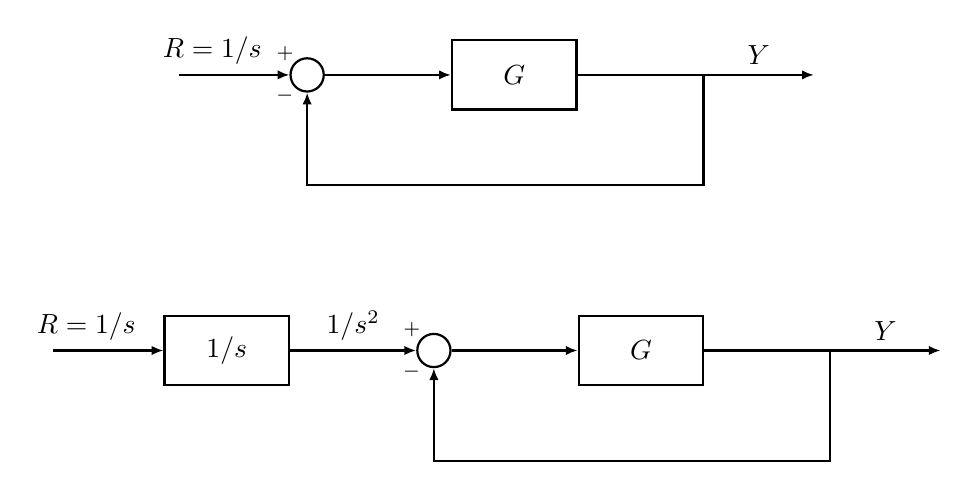
\begin{tikzpicture}[
  >={Latex[length=1.5mm, width=1.2mm]}, thick,
  block/.style = {draw, rectangle, minimum height=2.5em, minimum width=4.5em},
  sum/.style   = {draw, circle, inner sep=0pt, minimum size=1.2em},
]
  % ---- Top: step input drives the loop directly ----
  \node[coordinate]                       (rin1)  at (0, 0) {};
  \node[sum,   right=1.4cm of rin1]       (sum1)  {};
  \node[block, right=1.6cm of sum1]       (G1)    {$G$};
  \node[coordinate, right=1.6cm of G1]    (fbk1)  {};
  \node[coordinate, right=1.4cm of fbk1]  (yout1) {};

  \node[font=\scriptsize, inner sep=0pt, anchor=south east] at (sum1.north west) {$+$};
  \node[font=\scriptsize, inner sep=0pt, anchor=north east] at (sum1.south west) {$-$};

  \draw[->] (rin1) -- node[above, pos=0.3]{$R = 1/s$} (sum1);
  \draw[->] (sum1) -- (G1);
  \draw     (G1)   -- (fbk1);
  \draw[->] (fbk1) -- node[above]{$Y$} (yout1);

  \draw[->] (fbk1) -- ++(0,-1.4) -| (sum1.south);

  % ---- Bottom: step passes through an integrator first ----
  % rin2 shifted left by 1.6cm so the bottom diagram is centered horizontally
  % under the top.  (Bottom is wider by 3.2cm = integrator block + extra gap.)
  \node[coordinate]                       (rin2)  at (-1.6, -3.5) {};
  \node[block, right=1.4cm of rin2]       (int2)  {$1/s$};
  \node[sum,   right=1.6cm of int2]       (sum2)  {};
  \node[block, right=1.6cm of sum2]       (G2)    {$G$};
  \node[coordinate, right=1.6cm of G2]    (fbk2)  {};
  \node[coordinate, right=1.4cm of fbk2]  (yout2) {};

  \node[font=\scriptsize, inner sep=0pt, anchor=south east] at (sum2.north west) {$+$};
  \node[font=\scriptsize, inner sep=0pt, anchor=north east] at (sum2.south west) {$-$};

  \draw[->] (rin2) -- node[above, pos=0.3]{$R = 1/s$} (int2);
  \draw[->] (int2) -- node[above]{$1/s^2$}            (sum2);
  \draw[->] (sum2) -- (G2);
  \draw     (G2)   -- (fbk2);
  \draw[->] (fbk2) -- node[above]{$Y$}                (yout2);

  \draw[->] (fbk2) -- ++(0,-1.4) -| (sum2.south);
\end{tikzpicture}
\end{document}
